%!TEX root = ../dokumentation.tex

\chapter{Dockerfile}
\label{ch:Dockerfile}
Das Dockerfile (vgl. \autoref{fig:Dockerfile}) legt das Image für die später folgenden Anwendungscontainer fest. Der Dockercompose-Bereich \glqq  microservice-web\grqq{} (vgl. \autoref{fig:Docker-Compose-File}) und der dortige \glqq  build\grqq -Befehl referenzieren auf dieses Dockerfile.

\begin{wrapfigure}{r}{0\textwidth}
\centering
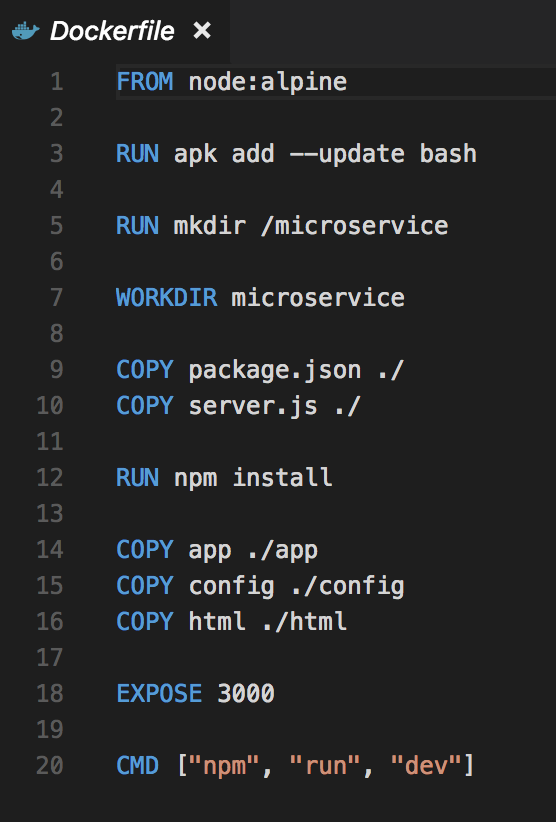
\includegraphics[height=.6\textwidth]{Dockerfile.png}
\vspace{3pt}
\caption{Dockerfile}
\label{fig:Dockerfile}
\end{wrapfigure}

Zeile 1: \textit{FROM} node:alpine legt das Betriebssystem des Containers fest. Hier wird auf eine Alpine-Maschine mit vorinstalliertem Node.js zurückgegriffen. Dieses System ist sehr beliebt für einfache Anwendungen und wird häufig für kleine Projekte verwendet, da es sehr geradlinig aufgebaut ist und wenig Ressourcen benötigt.

Zeile 3: \textit{RUN} beschreibt eine Eingabe in die virtuelle Kommandozeile. \glqq  apk add --update bash\grqq{} installiert die aktuelle Version von bash auf dem containerisierten Betriebssystem.

Zeile 5 bis Zeile 10: Die folgenden Kommandos erstellen einen Ordner auf dem Container, ändern das Arbeitsdirectory auf den neu erstellten Ordner und kopieren die Dateien \glqq package.json\grqq{} und \glqq server.js\grqq{} von der Festplatte des Aufrufers in den neu erstellten Ordner des Containers.

Zeile 12: \glqq npm install\grqq{} führt die Installation der Dependencies aus der kopierten \glqq package.json\grqq{} aus.

Zeile 14 bis Zeile 16: Die hier folgenden \textit{COPY}-Befehle kopieren die Ordner \textit{app}, \textit{config} und \textit{html} vom Host auf den Container.

Zeile 18: \textit{EXPOSE} beschreibt den Port auf den der Container später hört.

Zeile 20: Das Kommando \textit{CMD} beschreibt die final ausgeführten Befehle. In diesem Fall \glqq npm run dev\grqq{} welches in der \glqq package.json\grqq{} festgelegt wurde und die Anwendung im Development-Modus startet. An dieser Stelle könnte ebenfalls ein Releasekommando eingeführt werden.